\section{Профиль и протокол}
\subsection{Цель и теория}
Цель --- установить, даёт ли структура рёбер сведения сверх признаков вершин, и отделить чрезмерное сглаживание от плохой обучаемости~\cite{teacher}. Графовая сеть обновляет вершину агрегированными сообщениями соседей. После $L$ слоёв её рецептивное поле ограничено расстоянием $L$, но достижимость не гарантирует сохранения информации.
\begin{equation}\tilde A=A+I,\quad \tilde D_{ii}=d_i+1,\quad \hat A=\tilde D^{-1/2}\tilde A\tilde D^{-1/2},\qquad H^{l+1}=\sigma(\hat AH^lW^l).\end{equation}
Это GCN. В последнем слое ReLU отсутствует. При пустом графе $\hat A=I$ и слой совпадает с MLP с теми же весами. GAT заменяет фиксированные веса соседей обучаемыми нормированными коэффициентами $\alpha_{ij}\propto\exp(\operatorname{LeakyReLU}(a^\top[Wh_i;Wh_j]))$, включая петлю.

Гомофилия и два случайных ориентира определены как
\begin{equation}h_E=\frac{|\{(i,j)\in E:y_i=y_j\}|}{|E|},\quad h_0=\sum_c(N_c/N)^2,\quad h_{deg}=\sum_c(\operatorname{vol}_c/(2|E|))^2.\end{equation}
При независимом удалении рёбер с вероятностью $p$ ожидаемое число изолированных вершин равно $\sum_i p^{d_i}$. Degree-preserving null строится двойными перестановками рёбер без петель и повторов: он сохраняет все степени, но меняет соседей.

Для диагностики используются средний косинус $S$ на 20 000 фиксированных пар, val accuracy линейного probe и нормированная энергия Дирихле
\begin{equation}\hat E(H)=\frac{\operatorname{tr}(H^\top(I-\hat A)H)}{\|H\|_F^2}.\end{equation}
Без весов $\hat A^LX$ сходится внутри каждой компоненты к строкам вида $\sqrt{d_i+1}\,v$. Поэтому степень учитывается в энергии; простое равенство строк на нерегулярном графе не обязано давать ноль.

\subsection{Данные и настройки}
Персональный профиль: Cora, вторая GNN --- GAT, глубины 2,3,6,12,24. Использованы стандартные PyG Planetoid public masks: train 140, val 500, test 1000; cal пуст. Режим трансдуктивный: доступны X и рёбра всех вершин, но loss использует только train-метки, выбор параметров и checkpoint --- только val.

Исходный граф: 2708 вершин, 5278 неориентированных рёбер без петель и повторов, 1433 признака, семь классов, 78 компонент, изолированных вершин нет. Средняя степень 3.89808, медиана 3, максимум 168. $h_E=0.809966$, $h_0=0.179568$, $h_{deg}=0.169847$. Все метки используются только для описательных статистик гомофилии, не для выбора модели.

Основные модели имеют глубину 2, ширину 64, dropout 0.5, Adam, 200 эпох и полный batch единственного графа. У GAT восемь скрытых голов по восемь признаков. Общая сетка LR $\{0.01,0.005\}$ и weight decay $\{0.0005,0.005\}$. Выбраны: MLP 0.01/0.005, GCN и GAT 0.01/0.0005. При равной val accuracy выбирается ранняя эпоха. Все формальные модели обучены на CPU, два потока, float32. Ширина 16 используется только для отдельной проверки опубликованного ориентира.

\section{E1. Помогает ли граф}
\begin{table}[H]\centering\small
\setlength{\tabcolsep}{4pt}
\caption{E1: выбранные по val модели; accuracy в долях.}\label{tab:models}
\begin{tabular}{lrrrrrl}
\toprule
Модель & Train & Val & Test & Эпоха & $G_{top}$ & Ист. \\
\midrule
MLP & 1.0000 & 0.6320 & 0.6100 & 168 & +0.0000 & R01 \\
GCN & 0.9786 & 0.8160 & 0.8290 & 48 & +0.2190 & R02 \\
GAT & 0.9786 & 0.8120 & 0.8080 & 48 & +0.1980 & R03 \\
\bottomrule
\end{tabular}
\end{table}


GCN превосходит MLP на 0.2190, GAT --- на 0.1980. Отдельная GCN ширины 16 дала 0.8170: отклонение от ориентира 0.815 составляет 0.2 процентного пункта и укладывается в допуск 3 пункта. Сам по себе положительный $G_{top}$ ещё не выделяет пользу конкретных рёбер.
\begin{table}[H]\centering\footnotesize
\setlength{\tabcolsep}{4pt}
\caption{Удаление рёбер: A --- фиксированные веса, B --- переобучение на повреждённом графе.}\label{tab:deletion}
\begin{tabular}{rrrrrrl}
\toprule
$p$ & $M_A$ & $M_B$ & $N_{iso}$ & $\mathbb E N_{iso}$ & $h_E$ & Ист. A/B \\
\midrule
0 & 0.8290 & 0.8290 & 0 & 0.00 & 0.8100 & R02/R02 \\
0.1 & 0.8240 & 0.8140 & 51 & 54.92 & 0.8074 & R04/R05 \\
0.3 & 0.8090 & 0.8060 & 206 & 216.85 & 0.8073 & R06/R07 \\
0.5 & 0.7710 & 0.7710 & 478 & 493.47 & 0.8115 & R08/R09 \\
0.8 & 0.7340 & 0.6890 & 1343 & 1366.67 & 0.8111 & R10/R11 \\
1 & 0.7290 & 0.6050 & 2708 & 2708.00 & n/a & R12/R13 \\
\bottomrule
\end{tabular}
\end{table}


\begin{figure}[H]\centering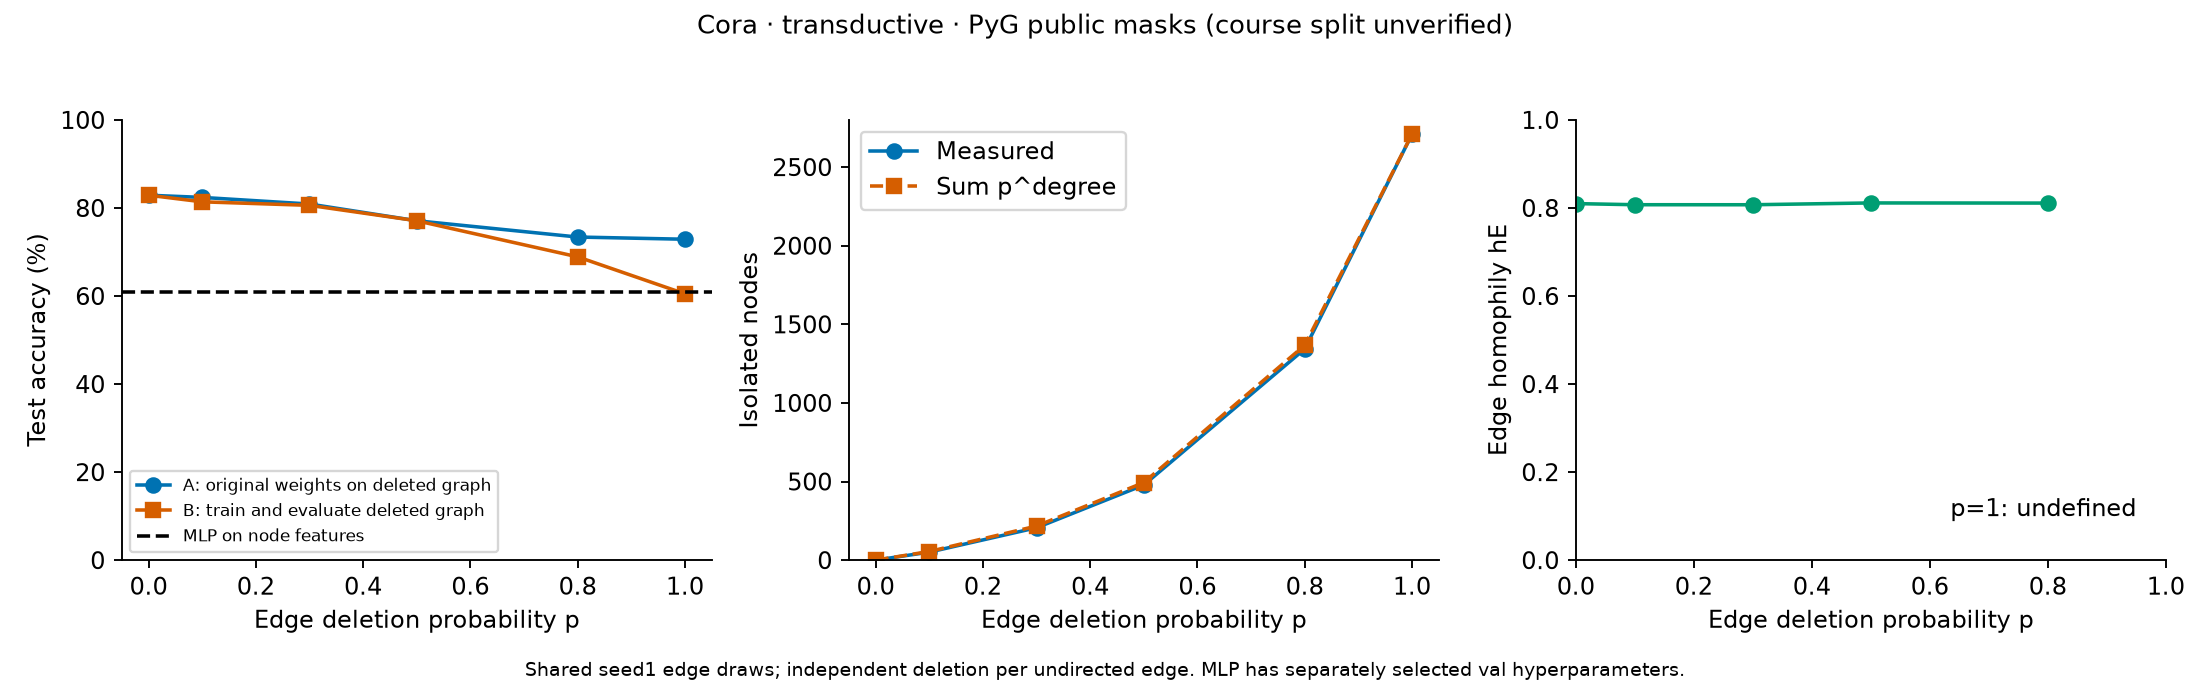
\includegraphics[width=\linewidth,height=.35\textheight,keepaspectratio]{figures/deletion.png}
\caption{E1: два режима удаления рёбер; трансдуктивная оценка.}\label{fig:deletion}
\end{figure}

Для $p=0.3,0.5,0.8$ относительные отклонения числа изолированных вершин от предсказания составили 5.00\%, 3.13\%, 1.73\%, меньше 20\%. Гомофилия оставшихся рёбер близка к исходной: случайное удаление уменьшает число соседей, а не систематически меняет долю внутриклассовых связей.

Кривая переобучения B впервые опускается до MLP на $p=1$: 0.6050 против 0.6100; все 1000 test-вершин изолированы. Разница 0.005 не противоречит тождеству слоёв при пустом графе: MLP и GCN имеют отдельно выбранные по val штрафы и checkpoint. Режим A при $p=1$ даёт 0.7290, поскольку веса были обучены на исходной структуре.

\section{E2. Конкретная структура рёбер}
До запусков зафиксировано ожидание положительной разности GCN на исходном графе и degree-preserving null величиной 15--35 процентных пунктов. Меняется только граф; X, masks, глубина 2, LR, weight decay и 200 эпох фиксированы. Общий seed задаёт инициализацию, dropout и нулевой граф; $Q=10$ попыток на каждое исходное ребро. Случай seed 1 с исходным графом ранее исследовался в E1, поэтому главный вывод не заявляется как полностью независимое подтверждение.
\begin{table}[H]\centering\footnotesize
\setlength{\tabcolsep}{4pt}
\caption{E2: GCN на исходном графе и degree-preserving null, три общих seed.}\label{tab:paired}
\begin{tabular}{rrrrrrrl}
\toprule
Seed & Исходный & Null & MLP & $\Delta_s$ & $h_{E,null}$ & Swap & Ист. G/null \\
\midrule
1 & 0.8290 & 0.3250 & 0.6100 & 0.5040 & 0.1635 & 0.9805 & R14/R15 \\
2 & 0.8210 & 0.3280 & 0.6110 & 0.4930 & 0.1646 & 0.9800 & R16/R17 \\
3 & 0.8200 & 0.3190 & 0.6020 & 0.5010 & 0.1701 & 0.9808 & R18/R19 \\
\bottomrule
\end{tabular}
\end{table}


\begin{figure}[H]\centering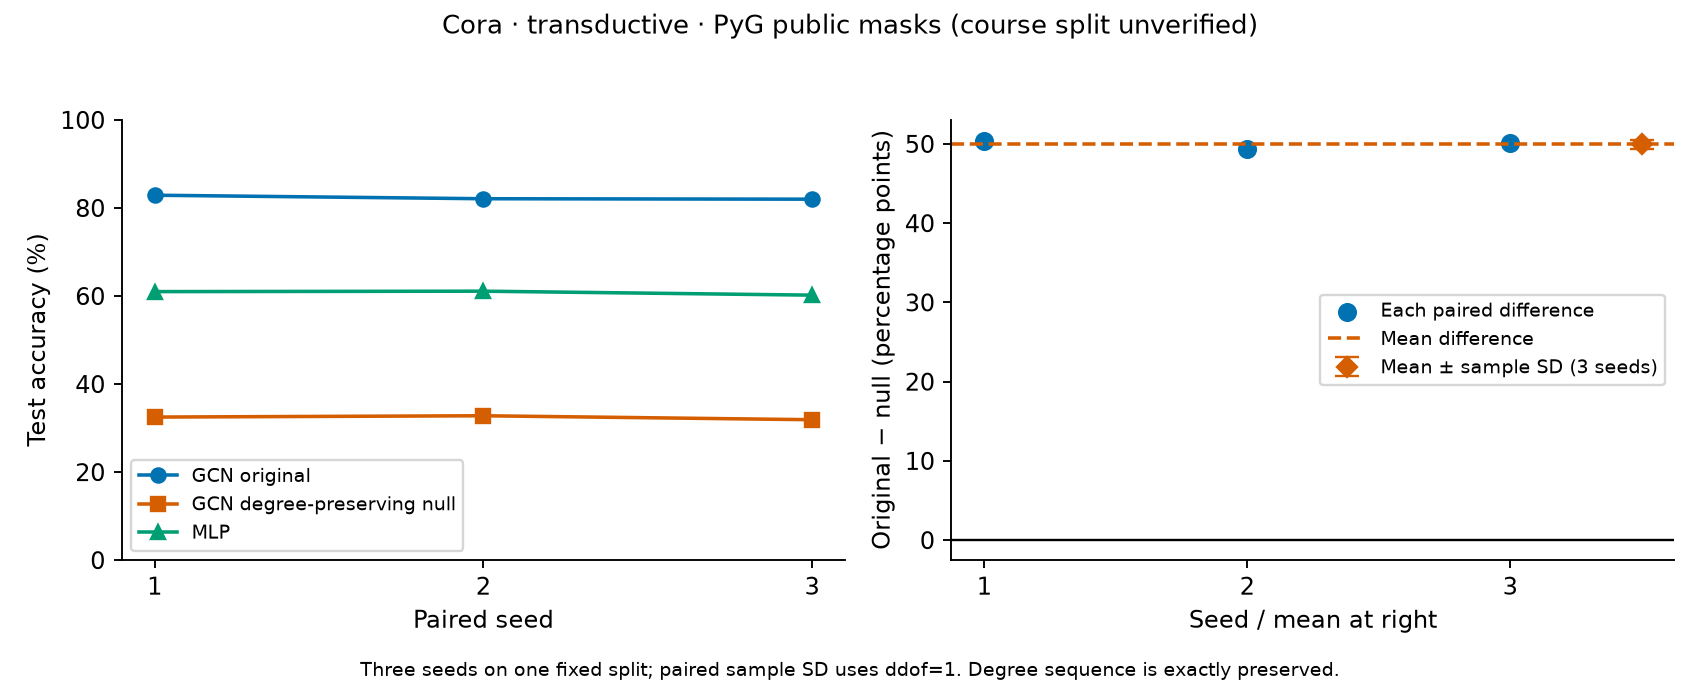
\includegraphics[width=\linewidth,height=.35\textheight,keepaspectratio]{figures/paired.png}
\caption{E2: точности и парные разности исходного и нулевого графов.}\label{fig:paired}
\end{figure}

Степени сохранены, успешны около 98\% перестановок. Значения $h_E$ null близки к $h_{deg}$ с отклонением менее 20\%. Все три разности положительны: 0.5040, 0.4930, 0.5010; среднее 0.499333, выборочное SD 0.005686. $|\bar\Delta|\ge2s_\Delta$, различие установлено: конкретная структура рёбер важна. Направление ожидания поддержано, количественный прогноз 0.15--0.35 не подтвердился. Случайные соседи не просто устраняют пользу рёбер: они способны ухудшить представление относительно MLP.

На графе Эрдёша--Реньи с тем же числом рёбер GCN seed 1 дала 0.3010, ниже degree null 0.3250. ER меняет степени, однако один такой результат не изолирует причинный вклад степени. Три seed E2 описывают неопределённость только на одном фиксированном split.

\section{E3. Глубина и сглаживание}
До обучения рассмотрено распространение $\hat A^lX$, $l=0,\ldots,24$: энергия убывает. В обученных plain GCN нет остатка и нормализации. По val лучшая глубина $l^*=2$. SD val accuracy трёх исходных GCN E2 равно $s_m=0.005292$; заметное падение --- больше $2s_m=0.010583$.
\begin{table}[H]\centering\scriptsize
\setlength{\tabcolsep}{4pt}
\caption{E3: выбранные checkpoint; показатели обучаемости и выходного представления.}\label{tab:depths}
\begin{tabular}{rrrrrrrrrl}
\toprule
$L$ & Train & Val & Test & $\rho_T$ & GI & $S$ & $\hat E$ & Probe & Ист. \\
\midrule
2 & 0.9786 & 0.8160 & 0.8290 & 0.2585 & 1.6077 & 0.1279 & 0.0638 & 0.7960 & R20 \\
3 & 1.0000 & 0.8120 & 0.8200 & 0.0200 & 1.2952 & 0.1658 & 0.0356 & 0.7920 & R21 \\
6 & 0.9571 & 0.7100 & 0.7010 & 0.1209 & 1.2851 & 0.2759 & 0.0206 & 0.7020 & R22 \\
12 & 0.1857 & 0.2700 & 0.2730 & 0.9965 & 6.1181 & 0.5658 & 0.6793 & 0.2100 & R23 \\
24 & 0.1571 & 0.2340 & 0.2090 & 0.9801 & 9.2301 & 0.7178 & 0.5704 & 0.1760 & R24 \\
\bottomrule
\end{tabular}
\end{table}


\begin{figure}[H]\centering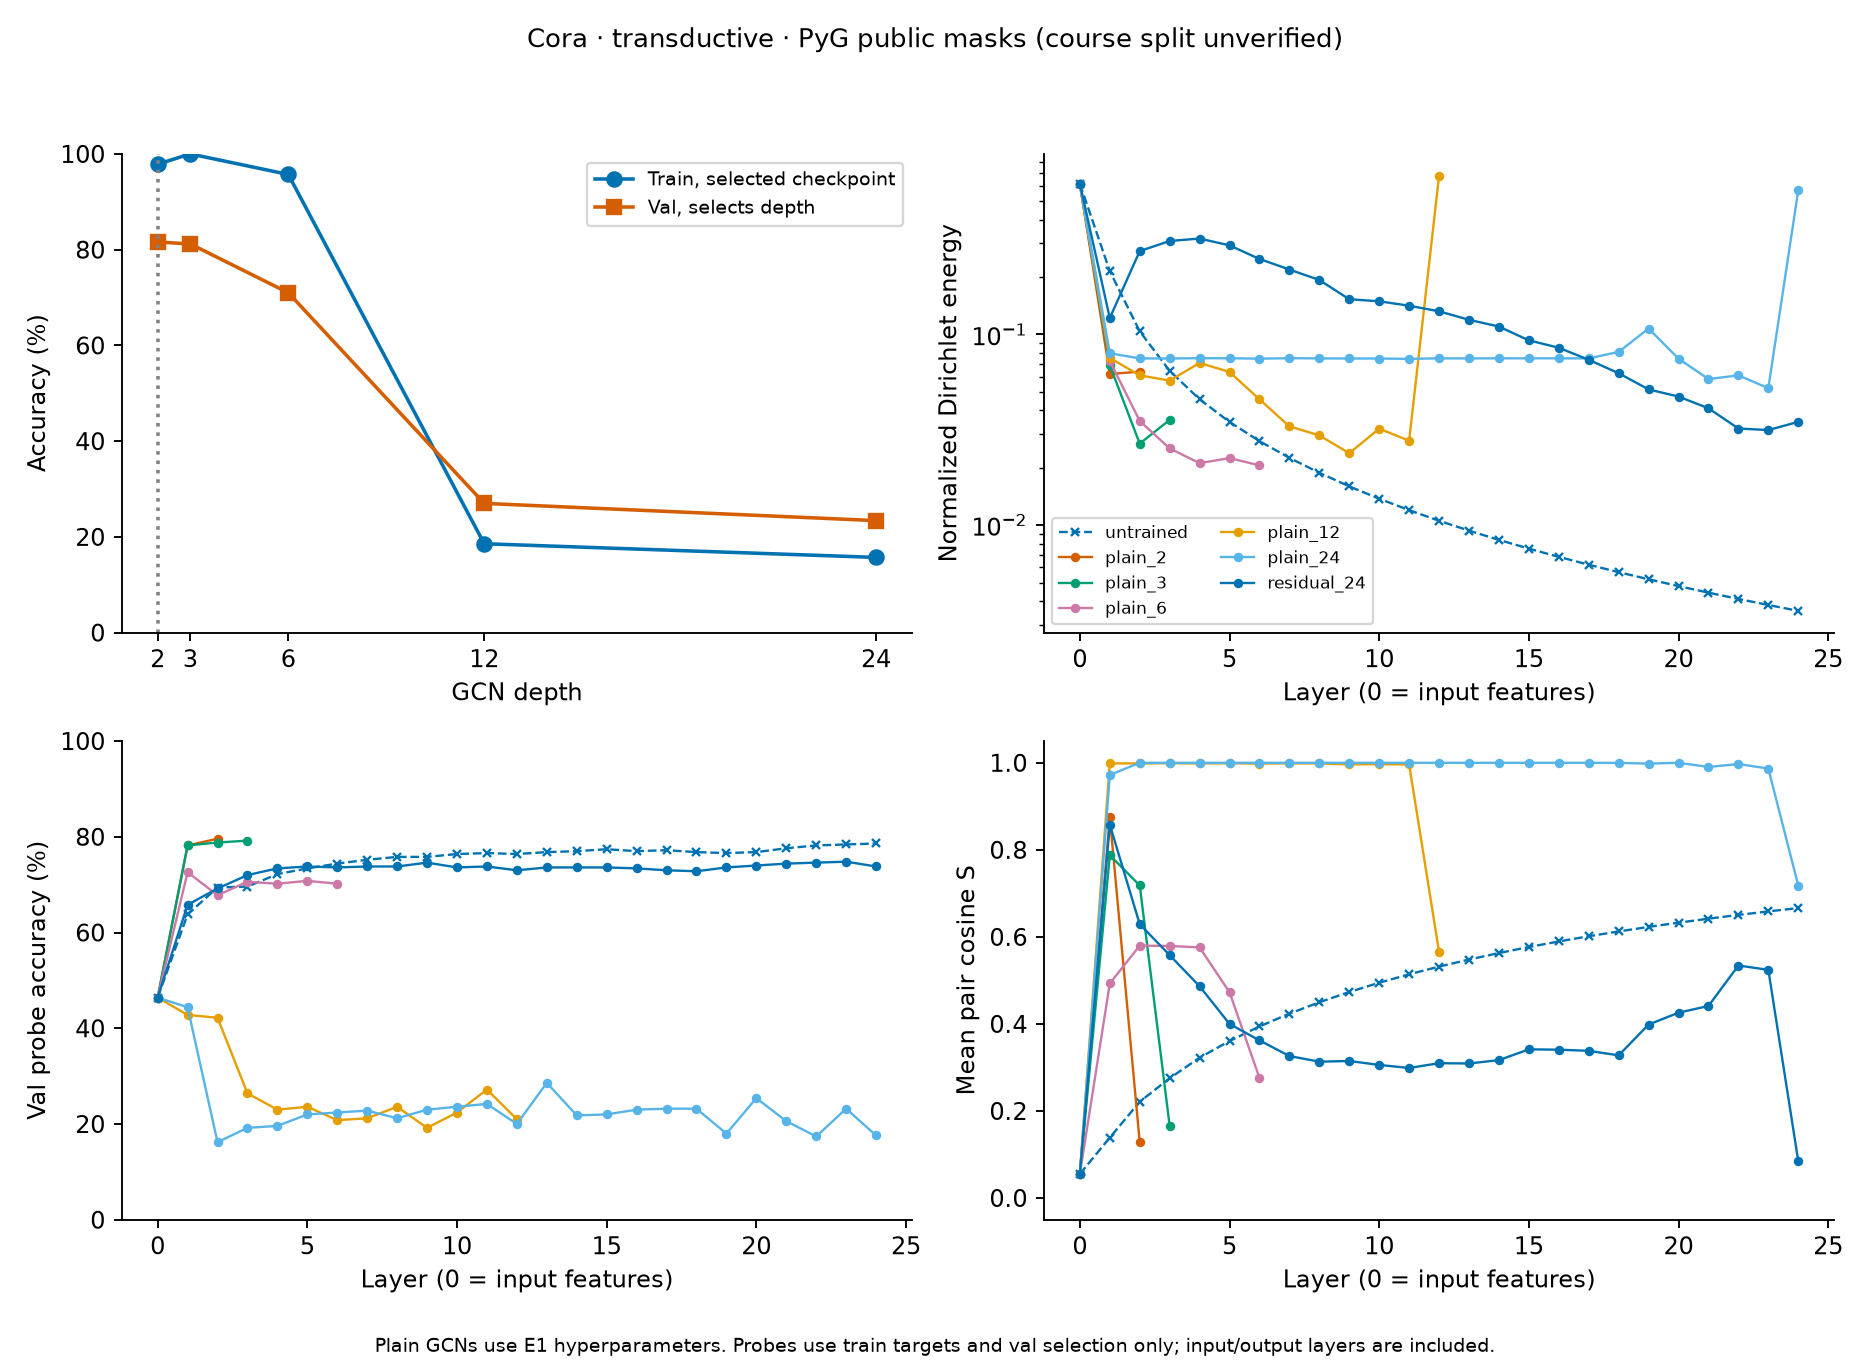
\includegraphics[width=\linewidth,height=.49\textheight,keepaspectratio]{figures/layers.png}
\caption{E3: точности по глубине, энергия, косинус и val-probe по слоям.}\label{fig:layers}
\end{figure}

При 6 слоях сеть обучилась ($\rho_T=0.120879$), энергия 0.020570 и probe 0.7020 ниже двухслойных 0.063777 и 0.7960. Совокупность признаков соответствует вредному сглаживанию. При 12 и 24 слоях $\rho_T\ge0.9$, train accuracy близка к случайной и GI большой: прежде всего это плохая обучаемость, а не доказанное сглаживание. Конвенция GI$\ge6$ использована как аналитический ориентир, численного порога GI преподаватель не задаёт. Таблица показывает диагностику выбранного checkpoint в eval по train; она не смешивается с медианой градиентов по всему обучению.

Обученная сеть имеет меньшую энергию, чем безвесовое распространение, при 2,3,6 слоях: 0.063777/0.103768, 0.035624/0.064405, 0.020570/0.027572. При 12,24 --- большую: 0.679321/0.010541, 0.570380/0.003551. Отношения описывают энергию, а не причину неудачного обучения.
\begin{figure}[H]\centering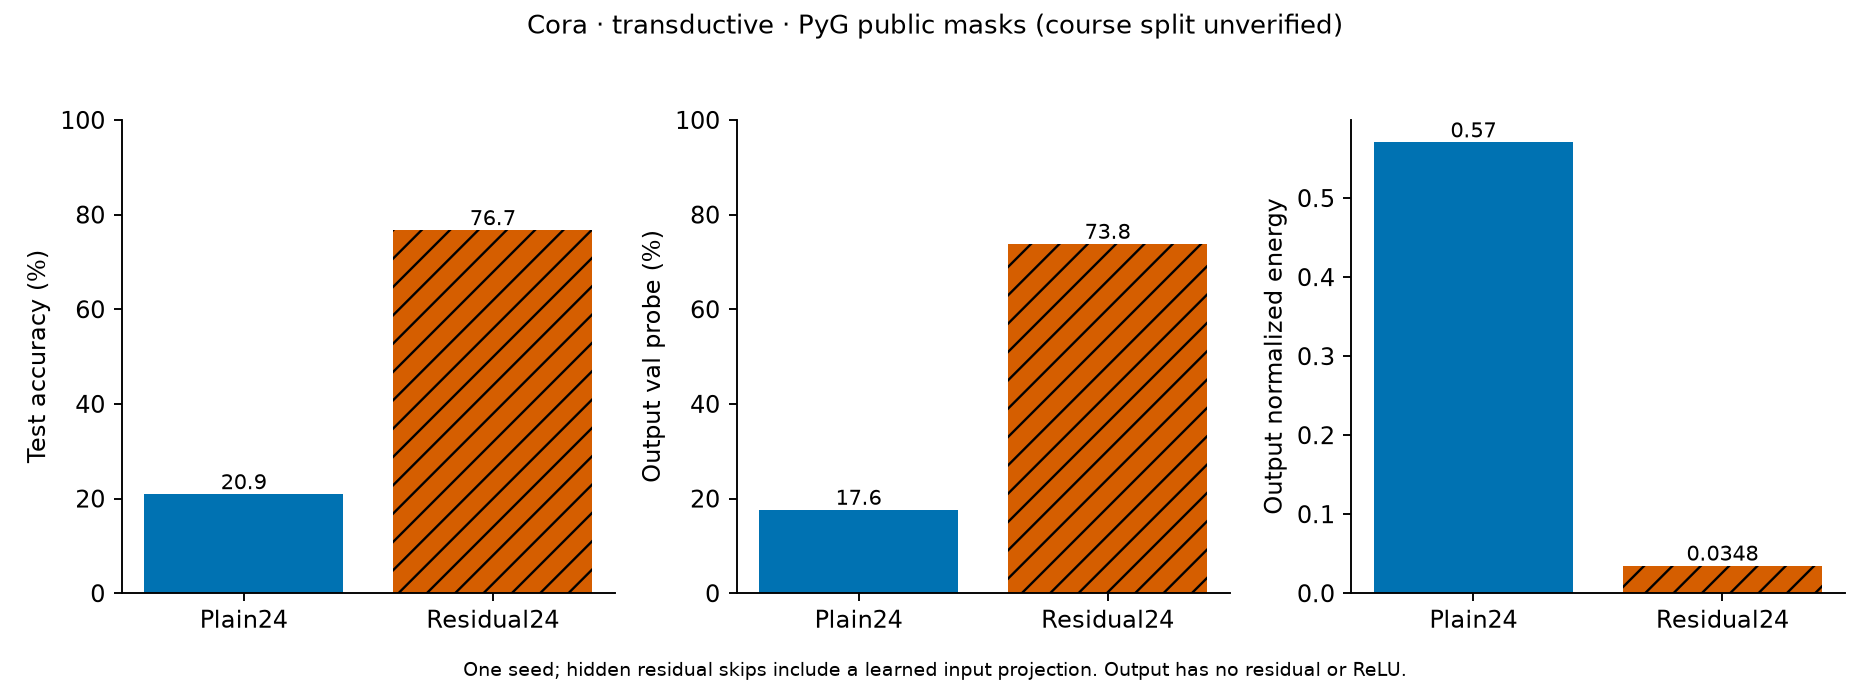
\includegraphics[width=\linewidth,height=.36\textheight,keepaspectratio]{figures/residual.png}
\caption{Граница применимости: 24 слоя без остатка и с остатком.}\label{fig:residual}
\end{figure}

24 слоя с остатком дали train/val/test 1.0000/0.7680/0.7670, $\rho_T=0.00529$, GI 1.5650, $S=0.08443$, $\hat E=0.034786$, probe 0.7380. При смене размерности используется обучаемая проекция, затем identity skip, выход без skip/ReLU. Предел $\hat A^LX$ к этой нелинейной обученной рекурсии прямо не применим.

\section{Карта зависимости качества от структуры}
\begin{table}[H]\centering\footnotesize
\setlength{\tabcolsep}{4pt}
\caption{Карта зависимости от структуры: seed 1, фиксированные X и маски.}\label{tab:map}
\begin{tabular}{lrrrrl}
\toprule
Условие & $L$ & Train & Val & Test & Ист. \\
\midrule
Исходный граф & 2 & 0.9786 & 0.8160 & 0.8290 & R02 \\
Удалено 50\% & 2 & 1.0000 & 0.7720 & 0.7710 & R09 \\
Без рёбер & 2 & 1.0000 & 0.6300 & 0.6050 & R13 \\
Degree null & 2 & 0.9857 & 0.3540 & 0.3250 & R15 \\
Эрдёш--Реньи & 2 & 1.0000 & 0.3300 & 0.3010 & R25 \\
Лучшая глубина & 2 & 0.9786 & 0.8160 & 0.8290 & R20 \\
Максимальная глубина & 24 & 0.1571 & 0.2340 & 0.2090 & R24 \\
MLP & 2 & 1.0000 & 0.6320 & 0.6100 & R01 \\
24 слоя с остатком & 24 & 1.0000 & 0.7680 & 0.7670 & R26 \\
\bottomrule
\end{tabular}
\end{table}


Фиксированы Cora, X, masks, 200 эпох, Adam и правило val checkpoint. Прямое сравнение графов использует одну GCN с фиксированными LR/штрафом; сравнение глубин меняет только глубину plain GCN. MLP и residual --- отдельные архитектурные ориентиры, поэтому карта не трактуется как однофакторный эксперимент целиком.

\section{Ответы на контрфактические вопросы}
\subsection*{Вопрос 1. Null и собственные признаки}
Seed 1: MLP 0.6100, null GCN 0.3250, null GAT 0.2690 (R27). Собственный коэффициент GCN равен $1/(d_i+1)$: при степенях 1,3,168 это 0.5,0.25,0.005917. Случайные соседи разбавляют собственные признаки. GAT может ослаблять соседей вниманием, но не обязан полностью их отвергать; наблюдаемое отличие GAT минус null GCN равно $-0.0560$. Оно не доказывает полезность случайных рёбер.
\subsection*{Вопрос 2. Добавление и удаление}
До построения графа предсказано $h'_E\approx(|E|h_E+2639h_0)/7917=0.599833$. Измерено 0.599217, ошибка $-0.000616$. Добавление 2639 случайных рёбер дало GCN test 0.7490 (R28), удаление примерно половины --- 0.7710. Добавление оказалось опаснее на 0.0220 в этом seed: оно снижает гомофилию и вводит чужие сообщения. Удаление преимущественно сохраняет гомофилию. Неопределённость одного сравнения не оценена.
\subsection*{Вопрос 3. Два режима удаления}
При $p=0.5$ оба режима дали 0.7710 против 0.8290 на исходном графе: падение 0.0580; изолированы 177 из 1000 test-вершин. Равные числа не означают равные механизмы: A проверяет сдвиг структуры при фиксированных весах, B позволяет адаптацию. Умеренное падение не доказывает, что граф не используется: остаются гомофильные соседи, признаки и петли.
\subsection*{Вопрос 4. Высокий косинус}
В первом слое plain GCN глубины 2 получены $S=0.875197$, $\hat E=0.061982$, probe 0.7820 при лучшем probe модели 0.7960 (R29). ReLU создаёт общее положительное направление, а косинус не отражает масштаб и небольшие различающие направления. Высокий $S$ сам по себе недостаточен; энергия оценивает соседское выравнивание с поправкой на степень, probe --- сохранение классовой информации.
\subsection*{Вопрос 5. Выбор глубины по test}
После фиксации выбора по val отдельно рассчитан posthoc argmax test: он тоже равен 2. Совпадение не делает выбор по test допустимым: трансдукция разрешает признаки и рёбра, но не использование test-меток для настройки. Исходный двухслойный test уже присутствовал в E1, поэтому не заявляется полностью невидимый test для этой глубины.

\noindent\textbf{Заключение.} На Cora конкретные рёбра дали устойчивый выигрыш над degree-preserving null. Шесть слоёв привели к вредному сглаживанию, 12 и 24 --- к плохой обучаемости; остаток улучшил обучение. Выводы относятся к данному split и рецепту.
\clearpage
\renewcommand{\refname}{Список использованных источников}
\begin{thebibliography}{9}
\addcontentsline{toc}{section}{Список использованных источников}
\bibitem{teacher} Лабораторная работа 5. Графовые нейронные сети. Насколько результат определяется структурой графа. Курс «Нейронные сети». Методические указания, 2026.
\end{thebibliography}
\clearpage
\section*{Приложение. Идентификация запусков}
\addcontentsline{toc}{section}{Приложение. Идентификация запусков}
\begingroup\small\setstretch{1.05}
\begin{longtable}{@{}l>{\raggedright\arraybackslash}p{3.5cm}p{10.8cm}@{}}
\caption{Полные RUN\_ID источников результатов.}\\
\toprule Код & Условие & RUN\_ID \\ \midrule \endhead
\hypertarget{R01}{R01} & E1 mlp & {\fontsize{8.8}{11}\selectfont\texttt{6dc64393605049154c62-e390858402844dfd8439193a33e59414}} \\
\hypertarget{R02}{R02} & E1 gcn & {\fontsize{8.8}{11}\selectfont\texttt{19bb59fb13252ba73de3-8e0a3696718f4ddeab1c9f002206edfb}} \\
\hypertarget{R03}{R03} & E1 gat & {\fontsize{8.8}{11}\selectfont\texttt{922f39512d2e378e6dbb-c3c1afd5768f4eafa3007b4ab4a1f32a}} \\
\hypertarget{R04}{R04} & delete A p0.1 & {\fontsize{8.8}{11}\selectfont\texttt{62a3f951f734211c790b-6dca5b96e4e44425b6e5796659c96566}} \\
\hypertarget{R05}{R05} & delete B p0.1 & {\fontsize{8.8}{11}\selectfont\texttt{7a06b6037c33f8a33db6-6e6f3e43e7f142aba33b93f2d03d250f}} \\
\hypertarget{R06}{R06} & delete A p0.3 & {\fontsize{8.8}{11}\selectfont\texttt{70e7e801068fbaa14e8f-9467fd3dd4ba44718b292b5c08203fc9}} \\
\hypertarget{R07}{R07} & delete B p0.3 & {\fontsize{8.8}{11}\selectfont\texttt{6de45895a645a6005574-2da6d1e8af83463083c3385dcf511764}} \\
\hypertarget{R08}{R08} & delete A p0.5 & {\fontsize{8.8}{11}\selectfont\texttt{03e1619b9899f2883b3d-e8688222db92423ab88987a7a88c7756}} \\
\hypertarget{R09}{R09} & delete B p0.5 & {\fontsize{8.8}{11}\selectfont\texttt{83bdc4e3aa823dd29101-0d25d7abb9e542859b180983675318bb}} \\
\hypertarget{R10}{R10} & delete A p0.8 & {\fontsize{8.8}{11}\selectfont\texttt{37127c5b272beb01e37c-e6ee9636a6e3437f91ba82ebb1a250f3}} \\
\hypertarget{R11}{R11} & delete B p0.8 & {\fontsize{8.8}{11}\selectfont\texttt{34e91694bbcc95320d27-0bfa21f151fc4ecb93ba45132b502497}} \\
\hypertarget{R12}{R12} & delete A p1 & {\fontsize{8.8}{11}\selectfont\texttt{58d3bc7f71ceff589bf7-671dd326e27249b8b7a9ad18f512935b}} \\
\hypertarget{R13}{R13} & delete B p1 & {\fontsize{8.8}{11}\selectfont\texttt{4d480d550deb7c01b60b-a2e9c042795a49348f137754b2faaeb7}} \\
\hypertarget{R14}{R14} & E2 G s1 & {\fontsize{8.8}{11}\selectfont\texttt{170997eb0516db15268e-bc9dd3adb6484c389e2394bef1c25035}} \\
\hypertarget{R15}{R15} & E2 null s1 & {\fontsize{8.8}{11}\selectfont\texttt{f1612dc13ae579d47fdc-1f33df1ac3aa47ec84dbd76b938a4bbc}} \\
\hypertarget{R16}{R16} & E2 G s2 & {\fontsize{8.8}{11}\selectfont\texttt{5e3dc7b2b4a8f04c4a58-eff300233e574c70a12504bbae61a014}} \\
\hypertarget{R17}{R17} & E2 null s2 & {\fontsize{8.8}{11}\selectfont\texttt{12f1a133897b3514871e-78d2f0eafae24f43afdb2e073cf08062}} \\
\hypertarget{R18}{R18} & E2 G s3 & {\fontsize{8.8}{11}\selectfont\texttt{9f9a170b0c7c29985d28-995dbbd00e024bfe9c0b8241a2a14def}} \\
\hypertarget{R19}{R19} & E2 null s3 & {\fontsize{8.8}{11}\selectfont\texttt{97644abed27cf38f5473-057f3aed2da14031bce8c388124d7535}} \\
\hypertarget{R20}{R20} & E3 depth2 & {\fontsize{8.8}{11}\selectfont\texttt{e5ad68ca624d0add75bb-bff2432311f343f38cc3b99ea9cb6706}} \\
\hypertarget{R21}{R21} & E3 depth3 & {\fontsize{8.8}{11}\selectfont\texttt{dc798ebb889c12508ca1-4181225ecd5749a89b607ef6adcf12a3}} \\
\hypertarget{R22}{R22} & E3 depth6 & {\fontsize{8.8}{11}\selectfont\texttt{55f726aa5ad6110db52f-4be93b2939ec4cf486e46c79f956fcff}} \\
\hypertarget{R23}{R23} & E3 depth12 & {\fontsize{8.8}{11}\selectfont\texttt{e419bb0c9f4ea256ac1a-425b7d8b9307440cb45c9e0d132fa69b}} \\
\hypertarget{R24}{R24} & E3 depth24 & {\fontsize{8.8}{11}\selectfont\texttt{585876aa03341faa5aa8-c2c6fd3a6d7743218e7a3bdc52bbef2b}} \\
\hypertarget{R25}{R25} & ER & {\fontsize{8.8}{11}\selectfont\texttt{e1f9226c3807d9516799-e75943f539284dec846455ee78becf0f}} \\
\hypertarget{R26}{R26} & maximum residual & {\fontsize{8.8}{11}\selectfont\texttt{d2b7fd35c37f89ad6858-a757e668893346a79a82c1823e72216f}} \\
\hypertarget{R27}{R27} & CF1 GAT null & {\fontsize{8.8}{11}\selectfont\texttt{d4019e4d9ffc0f51ebad-da107eb6b1fc474bad480d4ee24e01f3}} \\
\hypertarget{R28}{R28} & CF2 added edges & {\fontsize{8.8}{11}\selectfont\texttt{804407ffb262222bf788-5188bcee62fe409d81452e808519f81b}} \\
\hypertarget{R29}{R29} & CF4 high cosine & {\fontsize{8.8}{11}\selectfont\texttt{49dc168afb79b6fc9815-380db0ebe0084bc0957d925932b8d12a}} \\
\bottomrule\end{longtable}\endgroup
